\documentclass[11pt]{article}

\usepackage{amsmath}
\usepackage{amssymb}
\usepackage[linguistics]{forest}
\usepackage{mathtools}
\usepackage{bbm}
\usepackage[utf8]{inputenc} % this is needed for umlauts
\usepackage[ngerman]{babel} % this is needed for umlauts
\usepackage[T1]{fontenc}
\usepackage{fancyhdr}
\usepackage[makeroom]{cancel}
\usepackage{tikz}
\usepackage{enumitem}
\usepackage{ulem}
\usepackage{graphicx}
\usepackage{bm}

\graphicspath{{images/}}
\setlength{\parindent}{0pt}

\expandafter\def\expandafter\normalsize\expandafter{%
    \normalsize
    \setlength\abovedisplayskip{20pt}
    \setlength\belowdisplayskip{15pt}
    \setlength\abovedisplayshortskip{15pt}
    \setlength\belowdisplayshortskip{13pt}
}

\input ulem.sty

\newlist{arrowlist}{itemize}{1}
\setlist[arrowlist]{label=$\Rightarrow$}

\tikzset{node distance = 1cm and 5cm}
\usetikzlibrary{trees}
\usepackage[a4paper,bindingoffset=0.2in,
            left=1in,right=1in,top=1.2in,bottom=1in,
            footskip=.25in]{geometry}

\pagestyle{fancy}
\fancyhf{}
\rhead{\thesubsection}
\lhead{Experimentalphysik V}
\rfoot{Page \thepage}
\DeclareMathOperator*{\argmin}{arg\,min}
\DeclareMathOperator*{\argmax}{arg\,max}
\DeclarePairedDelimiter\ceil{\lceil}{\rceil}
\DeclarePairedDelimiter\floor{\lfloor}{\rfloor}
\DeclarePairedDelimiter\abs{\lvert}{\rvert}
\DeclarePairedDelimiter\norm{\lVert}{\rVert}
\DeclareMathOperator{\rank}{rank}


% Custom colors
\usepackage{color}
\definecolor{deepblue}{rgb}{0,0,0.5}
\definecolor{deepred}{rgb}{0.6,0,0}
\definecolor{deepgreen}{rgb}{0,0.5,0}

\usepackage{listings}

% Python style for highlighting
\newcommand\pythonstyle{\lstset{
language=Python,
basicstyle=\ttm,
otherkeywords={self},             % Add keywords here
keywordstyle=\ttb\color{deepblue},
emph={MyClass,__init__},          % Custom highlighting
emphstyle=\ttb\color{deepred},    % Custom highlighting style
stringstyle=\color{deepgreen},
frame=tb,                         % Any extra options here
showstringspaces=false            %
}}


% Python environment
\lstnewenvironment{python}[1][]
{
\pythonstyle
\lstset{#1}
}
{}

% Python for external files
\newcommand\pythonexternal[2][]{{
\pythonstyle
\lstinputlisting[#1]{#2}}}

% Python for inline
\newcommand\pythoninline[1]{{\pythonstyle\lstinline!#1!}}

\begin{document}
\section{Bindungstypen}
Die Bindungstypen unterscheiden sich vor allem durch die räumliche Verteilung
der Atome. Man findet diese Grundtypen im Allgemeinen nicht in reiner, sondern
in gemischter Form.
\begin{enumerate}
  \item \textbf{Van-der-Waals-Kraft} bei Festkörpern aus Molekülen oder
  Edelgasatomen
  \item \textbf{Ionenkristalle} Abgeschlossene Schalen, Elektronentransfer
  zwischen den Bindungspartnern
  \item \textbf{kovalente Bindungen} Valenzelelektronen zwischen den beteiligten
  Bindungspartnern lokalisiert
  \item \textbf{metallische Bindungen} Valenzelelektronen im Festkörper relativ
  gleichmäßig verteilt, starke 'Verschmierung' bewirkt Bindungskraft zwischen
  den Atomrümpfen und ermöglicht Leitfähigkeit
\end{enumerate}
\subsection{Van-der-Waals-Bindung}
\begin{itemize}
  \item Relevanz: neutrale Atome
  \item Schwach: $\sim$ 0.1eV/Atom
\end{itemize}
Wir addieren das anziehende Van-der-Waals-Potential zum abstoßenden Term durch
das Pauli-Prinzip und erhalten das Lennart-Jones-Potential:
\begin{equation}
  \phi (r) = \frac{A}{r^{12}} - \frac{B}{r^{6}} = 4 \varepsilon \left[ \left(
  \frac{\sigma}{r} \right )^{12} - \left ( \frac{\sigma}{r} \right )^6 \right ]
\end{equation}
Für die Bindungsenergie ergibt sich:
\begin{equation}
  U_B = \frac{1}{2} \sum_m \phi_m = \frac{N}{2} \phi_m = 2N\varepsilon \sum_{
  n \neq m} \left[ \left(
  \frac{\sigma}{r} \right )^{12} - \left ( \frac{\sigma}{r} \right )^6 \right ]
\end{equation}
\subsection{Ionenbindung}
Wenn wir die Ionen als geladenen Kugeln betrachten ergibt sich für die
Bindungsenergie:
\begin{equation}
  \phi = -\frac{e^2}{4\pi\varepsilon_0}\sim3-10\frac{eV}{Atom}
\end{equation}
Da die Ionen mit allen Nachbarn wechselwirken, erwarten wir im Festkörper
eine noch stärkere Bindung.
\subsection{Kovalente Bindung}
Die Elektronen sind nicht kugelförmig um den Kern verteilt. Es ergeben sich
zwei Zustände mit negativer und positiver Energieverschiebung, die als
anti-bindend bzw. bindend bezeichnet werden. Bei gebundenen Zuständen ist die
Aufenthaltswahrscheinlichkeit zwischen den Protonen höher, als man klassisch
erwarten würde. Für den nicht-bindenden Zustand ist sie null.
\subsection{Hybridorbitale}
Freie Kohlenstoffatome besitzen die Elektronenkonfiguration $1s^2 2s^2 2p^2$.
Zunächst erfolgt ein Übergang von der Konfiguration $2s^2 2p^2$ zu $2s 2p_x 2p_y
 2p_z$, was energetisch ungünstiger ist. Nun bilden sich aus den
Wellenfunktionen Linearkombinationen, die einen optimalen Überlapp mit
benachbarten Atomen ermöglichen. Die frei werdende Bindungsenergie kompensiert
den anfänglichen Energieverlust. Durch die lineare Überlagerung lassen sich
vier gleichwertige Wellenfunktionen definieren, die vom Zentrum eines Tetraeders
in alle vier Ecken weisen.
\subsection{Metallische Bindungen}
In Metallen sind die Valenzelelektronen weitgehend delokalisiert, also
gleichmäßig über den Kristall verteilt.
\section{Molekülanregungen}
\subsection{Rotation}
Für die Rotationszustände eines Moleküls gilt folgende Energie:
\begin{equation}
  E=\frac{1}{2}I\omega^2=\frac{L^2}{2I}=\frac{J\cdot(J+1)\hbar^2}{2I}=hcBJ(J+1)
\end{equation}
mit dem Trägheitsmoment
\begin{equation}
  I=\frac{m_1m_2}{m_1+m_2}R^2
\end{equation}
und der sogennanten Rotationskonstante
\begin{equation}
  B=\frac{h}{8\pi^2cI}
\end{equation}
Für den Abstand zwischen zwei Rotationsniveaus $n, n+1$ gilt:
\begin{equation}
  \Delta E=(2+2n)hcB=(1+n)\frac{\hbar^2}{I}
\end{equation}
Er steigt also mit steigender Quantenzahl. Das Rotationsspektrum ist außerdem
von den Übergangswahrscheinlichkeiten zwischen den Zuständen abhängig. Wenn
diese ungefähr gleich sind, dan spiegeln die Intensitäten der Spektrallinien
die Besetzungsdichten wieder. Diese ist proportional zur Boltzman-Statistik:
\begin{equation}
  \frac{\mu_j}{\mu_0}=(2J+1)\cdot e^{-\frac{hcBJ(J+1)}{k_BT}}
\end{equation}
Der Faktor (2J+1) ergibt sich, da es sich bei dem Zustand mit der Quantenzahl J
eigentlich um (2J+1) Zustände handelt. Im unteren Bereich der Besetzung ist die
Entartung dominant, im oberen Bereich der exponentielle Abfall. Die Abstände
zwischen den Spektrallinien sind dabei alle gleich, da gilt:
\begin{equation}
  \Delta\Delta E=2hcB=\frac{\hbar^2}{I}
\end{equation}
Außerdem sind immer nur Übergänge zum nächstgelegenen Niveau möglich.

\subsection{Vibration}
Die Atome eines zweiatomigen, hantelförmigen Moleküls können auch gegeneinander
schwingen. Die einfachste Näherung ist eine harmonische Schwingung. Für die
Energieniveaus gilt:
\begin{equation}
  E_\mu=\hbar\omega_0\left(\mu+\frac{1}{2}\right)
\end{equation}
Die Auswahlregeln für den harmonischen Oszillator sind $\Delta\nu=\pm1$.
Für die Kraftkonstante der Molekülbindung gilt:
\begin{equation}
  \nu=\frac{1}{2\pi}\sqrt{\frac{k}{\mu}}
\end{equation}
\subsection{Elektronische Anregungen}
Eine molekulare Schwingung wird angeregt, wenn das Molekül ein Quant mit der
Energie $E=h\nu$ absorbiert. Der direkteste Weg den Schwingungszustand eines
Moleküls zu untersuchen, ist mithilfe der Infrarotspektroslopie, denn die zur
Anregung notwendige Energie entspricht bei den meisten Verbindungen der Energie
eines Photons im Infrarotbereich. Wechselwirkung zwischen elektromagnetischer
Strahlung und dem Molekül kann nur dann auftreten, wenn im Molekül bewegte
elektrische Ladung zur Verfügung steht. Das ist immer dann der Fall, wenn das
Molekül entweder ein veränderbares oder ein induzierbares Dipolmoment aufweist
(\textbf{IR-aktiv}). In Molekülen mit Schwingungen symmetrisch zum
Symmetriezentrum treten keine Änderungen des Dipolmomentes auf. Solche
'verbotenen' Schwingungen sind oft raman aktiv. Infrarot inaktiv sind
beispielsweise Moleküle wie $H_2, N_2, 0_2$, sie sind aber raman aktiv, weil
sich bei ihnen die Polarisierbarkeit ändert.
In der Infrarotspektroskopie treten keine reinen Schwingungen auf. Die Energie,
die zu einer Anregung einer Schwingung aufgebracht werden muss, reicht immer,
um Rotationsübergände von Molekülen hervorzurufen. Man spricht von
Rotationsschwingungsspektren. Die Gesamtenergie kann man nun als Summe der
Energie der Rotation und der Energie der Schwingung betrachten.
\begin{equation}
  E_{ges}=E_{vib}+E_{rot}
\end{equation}
\begin{equation}
  E_{ges}=\left(\mu+\frac{1}{2}\right)h\mu+hc_0BJ(J+1)
\end{equation}
Bei einem Schwingungsübergang ändern sich also gleichzeitig die
Rotationsübergänge um $\Delta J\pm1$. Wenn $\Delta J=+1$, spricht man vom
R-Zweig. Bei $\Delta J=-1$ spricht man vom P-Zweig. Übergänge mit $\Delta J=0$
sind verboten und werden Q-Zweig genannt.
Für die Frequenz eines Photons beim Übergang eines P-Zweiges gilt:
\begin{equation}
  \omega_P=\frac{E_{1,j-1}-E_{0,j}}{\hbar}=\omega_0+
  [J(J-1)-J(J+1)]\frac{\hbar^2}{2I}=\omega_0-\frac{J\hbar^2}{I}
\end{equation}
Bei einem Übergang des R-Zweiges ergibt sich:
\begin{equation}
  \omega_R=\frac{E_{1,j+1}-E_{0,j}}{\hbar}=\omega_0+[(J+1)(J+2)-J(J+1)]=
  \omega_0+(J+1)\frac{\hbar^2}{I}
\end{equation}

\section{Struktur von Festkörpern}
Kristalle zeichnen sich durch Translationssymmetrie aus:
\begin{equation}
  \mathcal{U}(r)= \mathcal{U}(\bm{r}+\bm{R})
\end{equation}
Die Translation wird durch den Gittervektor R beschrieben.
\begin{equation}
  \bm{R} = n_1\bm{a}+n_2\bm{b}+n_3\bm{c}
\end{equation}
Die Vektoren $\bm{a}, \bm{b}, \bm{c}$ bezeichnet man als Basisvektoren.
Die Längen a, b, c der Basisvektoren bezeichnet man als Gitterkonstanten. Das
Parallelepiped, das von den Basisvektoren aufgespannt wird, bezeichnet man als
Einheitszelle. Die Wahl der Basisvektoren ist nicht eindeutig. Man unterscheided
primitive und nicht-primitive Einheitszellen. \textbf{Primitive Elementarzellen}
sind die kleinstmöglichen Zellen und enthalten nur einen Gitterpunkt, den man
meist als Ursprung der Elementarzelle wählt. Mit den zugrundeliegenden
Basisvektoren können alle äquivalenten Raumpunkte erreicht werden.
\textbf{Nicht-primitive Elementarzellen} enthalten mehr als einen Gitterpunkt.
Ihre Basisvektoren erlauben nicht, alle äquivalenten Raumpunkte zu erreichen.
\subsection{Kubische Kristalle}
\begin{itemize}
  \item Simple cubic
  \item Face centered cubic (fcc)
  \item Body centered cubic (bcc)
\end{itemize}
Diese unterscheiden sich durch Zahl und Anordnung der Gitterpunkte und somit
auch durch ihre Packungsdichte. Die Kantenlänge des Würfels ist die
Gitterkonstante a.
Für die Packungsdichte gilt:
\begin{equation}
  P=\frac{N\cdot V_{\text{Atom}}}{V_{\text{Elementarzelle}}}
\end{equation}
\subsubsection{Simple cubic}
\begin{itemize}
  \item Sechs nächste Nachbarn im Abstand a
  \item Zwölf übernächste Nachbarn im Abstand $\sqrt{2}$a
  \item Packungsverhältnis: 0.52
  \item Simple cubic mit einatomiger Basis kommt in der Natur nur sehr selten
  vor, man findet es häufiger bei Kristallen mit mehratomiger Basis.
\end{itemize}
\subsubsection{Face centered cubic}
\begin{itemize}
  \item Edelgasmetalle und viele Legierungen besitzen diese Anordnung
  \item Die kubische Elementarzelle enthält vier Gitterpunkte
  \item Zwölf nächste Nachbarn im Abstand $\frac{a}{\sqrt{2}}$
  \item Sechs übernächste Nachbarn im Abstand a
  \item Packungsdichte von 0.74 (maximal). Es befinden sich 4 Kugeln in der
  Elementarzelle. Der größtmögliche Radius um die Atome ist $r=\frac{\sqrt{2}a}
  {4}$ und das Volumen der Elementarzelle ist $a^3$. Es folgt:
  \begin{equation}
    P=\frac{N\cdot\frac{4}{3}\pi r^3}{a^3}=
    \frac{4\cdot\frac{4}{3}\pi\left(\frac{\sqrt{2}a}{4}\right)^3}{a^3}
    \approx 0.7405
  \end{equation}
  \item Man könnte statt der kubischen (nicht primitiven) Elementarzelle auch
  einen Rhomboeder mit Kantenlänge $\frac{a}{\sqrt{2}}$ wählen, um eine
  primitive Einheitszelle zu bekommen.
  \item Beispiel: Diamant. Zweiatomige Basis mit Koordinaten (0, 0, 0),
  $(\frac{1}{4}, \frac{1}{4}, \frac{1}{4})$. Das Packungsverhältnis beträgt hier
  nur 0.34.
\end{itemize}
\subsubsection{Body centered cubic}
\begin{itemize}
  \item Viele Alkalimetalle besitzen diese Struktur
  \item Die Elementarzelle enthält zwei Gitterpunkte
  \item Acht nächste Nachbarn im Abstand $\frac{a\sqrt{3}}{2}$
  \item Sechs übernächste Nachbarn im Abstand a
  \item Packungsverhältnis: 0.68
  \item Man könnte statt der kubischen (nicht primitiven) Elementarzelle auch
  einen Rhomboeder mit Kantenlänge $\frac{a\sqrt{3}}{2}$ wählen, um eine
  primitive Einheitszelle zu bekommen.
\end{itemize}
\subsection{Wigner-Seitz-Zelle}
Die Wigner-Seitz-Zelle schließt den Raum ein, der dem ausgewählten Gitterpunkt
näher ist als jedem anderen Gitterpunkt. Um sie zu konstruieren, wird zunächst
ein Gitterpunkt mit seinen Nachbarn verbunden. Anschließend werden
Mittelsenkrechten auf diesen Verbindungsliniern eingezeichnet. Die so
konstruierte Elementarzelle ist primitiv und besitzt die volle Gittersymmetrie.
\section{Reziprokes Gitter}
Detaillierte Kentnisse über den Aufbau von Festkörpern wurden in erster Linie
mit Beugungsexperimenten gewonnen. Man lässt Wellen auf die Probe fallen, die
von den Atomen gestreut werden und beobachtet das Beugunsmuster. Davon kann
auf die geometrische Anordnung der Atome geschlossen werden. Für diese
Streuexperimente eignen sich Röntgenstrahlung, Elektronen, Neutronen oder
leichte Atome. Die Stärke der Wechselwirkung bestimmt die Eindringtiefe.
Elektronen oder Atomstrahlen eignen sich auf Grund der Coulomb-Wechselwirkung
vor allem zur Untersuchung von Oberflächen, Röntgen- und Neutronenstrahlen
dagegen zur Untersuchung massiver Festkörper, da die Neutronen bei Atomen ohne
magnetisches Moment ausschließlich an den Kernen gestreut werden. \textbf{
Beugung} ist besonders dann stark ausgeprägt, wenn die Lichtwellenlänge und die
charakteristische Länge des zu untersuchenden Objekts gleich lang sind.
Setzen wir eine Wellenlänge von 1 $\mathring{A}$ voraus, ergibt sich:
\begin{equation}
  E = \frac{p^2}{2m} = \frac{\hbar^2}{2\lambda^2m} = \frac{\hbar^2}{2
  \mathring{A}^2m}
\end{equation}
Somit haben Neutronen bei dieser Wellenlänge eine deutlich geringere Energie
als Lichtquanten oder Elektronen. Die Information über die Verteiung der
Streuzentren steckt im Integral
\begin{equation}
  \mathcal{A}(\bm{K})=\int_{V_P}\rho(r)e^{-i\bm{K}\cdot\bm{r}}dV
\end{equation}
wobei $\rho(r)$ die Streudichteverteilung ist und $\bm{K}=\bm{k}-\bm{k}_0$
der Streuvektor ist. Somit lässt dich über eine Fouriertransformation aus der
Streudichteverteilung der Streuvektor rekonstruieren. Wir schreiben nun:
\begin{equation}
  \rho(\bm{r})=\sum_{h,k,l}\rho_{hkl}e^{i\bm{G}_{hkl}\cdot\bm{r}}
\end{equation}
Für $G_{hkl}$ gilt weiter:
\begin{equation}
  G_{hkl}=h\bm{b}_1+k\bm{b}_2+l\bm{b}_3
\end{equation}
Die Vektoren $\bm{b}_1, \bm{b}_2, \bm{b}_3$ legen nun ein neues,
schiefwinkliges Koordinatensystem fest. Aus der Bedingung
\begin{equation}
  \rho(\bm{r})=\rho()\bm{r}+\bm{R})
\end{equation}
folgt:
\begin{equation}
  \bm{b}_i\cdot\bm{a}_j=2\pi\delta_{ij}
\end{equation}
Somit folgt für die rezproken Gittervektoren:
\begin{equation}
  \begin{align}
    \bm{b}_1&=\frac{2\pi}{V_Z}(\bm{a}_2\times\bm{a}_3) \\
    \bm{b}_2&=\frac{2\pi}{V_Z}(\bm{a}_3\times\bm{a}_1) \\
    \bm{b}_3&=\frac{2\pi}{V_Z}(\bm{a}_1\times\bm{a}_2) \\
  \end{align}
\end{equation}
Für das Volumen im reziproken Raum gilt:
\begin{equation}
  (\bm{b}_1\times\bm{b}_2)\cdot\bm{b}_3=\frac{(2\pi)^3}{V_Z}
\end{equation}
\subsection{Brillouin-Zonen}
Auch im reziproken Gitter lässt sich eine Wigner-Seitz Zelle konstruieren.
Diese heißt erste Brillouin-Zone und spielt eine wichtige Rolle bei der
Gitterdynamik. Brillouin-Zonen höherer Ordnung erhält man, indem man die
nächsten Nachbarn gegen weiter entfernte tauscht.
\subsection{Millersche Indize}
Wir betrachten eine Gitterebene, deren Achsenabschnitte wir in Einheiten
der Basisvektoren $a_i$ angeben. So erhalten wir beispielsweise 4, 2 und $\infty$
(wenn kein Achsenabschnitt auftritt). Nun bilden wir die Kehrwerte und erhalten
$\frac{1}{4}, \frac{1}{2}, 0$. Nun multiplizieren wir diese 3 Zahlen mit einem
Faktor m, der so gewählt wird, dass sich 3 ganze Zahlen ergeben. In unserem
Fall ist $m=4$ und wir erhalten für die Millerschen Indizes $(hkl)= (120)$. Mit
dieser Notation kann man auch Richtungen angeben. Die [hkl]-Richtung ist die
Richtung des Vektors $[hkl]=h\bm{a}_1+k\bm{a}_2+l\bm{a}_3$. Bei kubischen
Kristallen steht dieser Vektor senkrecht auf der [hkl]-Ebene.
\subsection{Experimentell Bestimmung der Kristall-Struktur}
Die Intensität der gestreuten Strahlung ist proportional zur Streu-Amplitude.
\begin{equation}
  \mathcal{I}(\bm{K}) \propto \abs{\mathcal{A}(\bm{K})}^2=
  \abs{\int_{V_P}\rho(\bm{r})e^{i\bm{K}\cdot\bm{r}}dV}^2
\end{equation}
Wenn wir nun die Entwicklung der Streudichteverteilung $\rho(\bm{r})$ nach den
Basisvektoren des reziproken Gitters einsetzen, erhalten wir:
\begin{equation}
  \abs{\mathcal{A}(\bm{K})}^2=\abs{\sum_{h,k,l}\rho_{hkl}\int_{V_P}
  e^{i(\bm{G}-\bm{K})\cdot\bm{r}}dV}^2
\end{equation}
Die Beträge mitteln sich bei der Integration weg, außer es gilt die
Beugungsbedingung:
\begin{equation} \label{ref1}
  \bm{K}=\bm{G}
\end{equation}
Hier nimmt die Exponentialfunktion den Wert 1 an, ein Ausdruck dafür, dass die
Überlagerung der Streuwellen konstruktiv erfolgt. Bei endlichem Probevolumen
oder endlicher Eindringtiefe ist die Streubedingung etwas aufgeweicht.
\subsection{Ewald-Kugel und Bragg-Bedingung}
Lässt man Strahlung mit dem Wellenvektor $\bm{k}_0$ auf einen Kristall fallen,
so tritt in den meisten Fällen keine Reflexion auf, da die Beugungsbedingung
nicht erfüllt ist. Bei vorgegebener Einfallsrichtung muss der Kristall passend
ausgerichtet werden, und die Beobachtung in der richtigen Richtung erfolgen.
Dazu stellt man das reziproke Gitter da und zeichnet den Vektor $k_0$ so ein,
dass sein Endpunkt in einem Punkt des Gitter liegt. Nun zieht man einen Kreis
mit dem Radius $k_0$ um den Urspung des Wellenvektors. So kennzeichnet man die
Menge aller Streuvektoren $\bm{K}=\bm{k}-\bm{k}_0$ für elastische Streuung
$\abs{\bm{k}}=\abs{\bm{k}_0}$. Die Streubedingung ist erfüllt, wenn die Ewald-
Kugel einen Punkt des reziproken Gitters berührt. In diesem Fall tritt ein
gebeugter Strahl in Richtung von $\bm{k}$ mit Wellenvektor $\bm{K}$ auf.
Wird ein Reflex beobachtet, dann ist über die Beugungsbedingung auch der
mitwirkende Gittervektor $\bm{G}$ mit dem Zahlentripel (hkl) festgelegt. Dies
bedeutet, dass die Streuung an einer periodischen Schwankung der Streudichte
erfolgt, deren Periode gegeben ist durch:
\begin{equation} \label{ref2}
  d_{hkl}=\frac{2\pi}{\abs{\bm{G}_{hkl}}}
\end{equation}
Ist $\theta$ der Winkel zwischen der Einfallsrichtung der Welle und den Ebenen
der streuenden Dichteschwankung, so gilt wegen $k_0=k$ für den Betrag des
Streuvektors:
\begin{equation}
  K = \abs{\bm{k}-\bm{k}_0}=2k_0\sin(\theta)=\frac{(4\pi\sin(\theta))}
  {\lambda}
\end{equation}
Setzt man diese Beziehung und Gleichung \ref{ref2} in Gleichung \ref{ref1} ein,
so erhält man die Bragg-Bedingung.
\begin{equation}
  2d_{hkl}\sin{\theta}=\lambda
\end{equation}
\section{Gitterdynamik}
Für die Geschwindigkeit longitudinaler Wellen gilt in Kristallen
\begin{equation}
  v_l=\frac{\omega}{q}
\end{equation}
\subsection{Gitterschwingungen}
Liegt ein Wellenvektor q' außerhalb der ersten Brillouin-Zone, so lässt er sich
durch Addition eines reziproken Gittervektors $\frac{2\pi p}{a}$ wieder in diese
zurückführen, wobei p für eine ganze Zahl steht. Eine Welle, die in Richtung der
positiven x-Achse läuft und deren Wellenvektor in der zweiten Brillouin-Zone
liegt, besitzt nach Addition des reziproken Gittervektors $\bm{G}=\frac{2\pi}
{a}$ einen Wellenvektor, der in die entgegengesetzte Richtung zeigt. Somit
ändert die Phasengeschwindigkeit $v=\frac{\omega}{q}$ ihr Vorzeichen. Die
Gruppengeschwindigkeit $v_g=\frac{\partial w}{\partial q}$ und damit der
Energietransport ändert sich hingegen nicht. An der Grenze der Brillouin-Zone
geht die Gruppengeschwindigkeit gegen null und es treten stehende Wellen auf.
\subsection{Gitter mit mehratomiger Basis}
Enthält die primitive Einheitszelle mehrere Atome, so treten neue Effekte auf.
Nach dem Lösen der Wellengleichung finden wir nun zwei Lösungen, den optischen
und den akkustischen Zweig. Die Gitterschwingungen einer linearen Kette mit
ein- oder zweiatomiger Basis unterscheiden sich also schon in der Anzahl der
Zweige. Der akkustische Zweig entspricht dem Verhalten einer einatomigen Kette.
Dies lässt sich zeigen, indem man $M=M_1=M_2$ annimmmt und den Gitterabstand
a durch 2a ersetzt.
\noindent \paragraph{Optischer Zweig} Für $q\to 0$ erhalten wir für die Phasen
u, v zweier Atome $\omega \approx 0$ und somit $u \approx v$. Für den optischen
Zweig finden wir hingegen $\frac{u}{v}=-\frac{M_2}{M_1}$. Dies bedeutet, dass
alle Atome mit der Masse $M_2$ in Gegenphase zu denen mit der Masse $M_1$
schwingen. Offensichtlich sind akkustische Gitterwellen bei langen Wellen $
q\to 0$ identisch mit Schallwellen. Bei den optischen Wellen ist mit der
gegenphasigen Auslenkung der Untergitter ein oszillierendes Dipolmoment
verknüpft, wenn die schwingenden Atome entgegengesetzte Ladung tragen. Dadurch
können die Schwingungen an elektromagnetische Wellen ankoppeln und bestimmen
die optischen Eigenschaften im Infrarotbereich (Bezeichnung: infrarotaktiv).
An der Grenze der Brillouin-Zone finden wir $\frac{v}{u}=0$, abgängig vom
betrachteten Zweig ist also das Untergitter der schweren oder der leichten
Atome in Ruhe, während der andere Teil des Gitters schwinkt. Für diese
Gitterschwingungen verschwindet also das oszillierende Dipolmoment, auf Grund
der gegenphasigen Schwingungen der Ionen in den benachbarten Zellen. Ist $M_1
\neq M_2$ so existiert an der Grenze der Brillouin-Zone eine \textbf{
Frequenzlücke}. In der verbotenen Zone existieren keine Eigenschwingungen des
Gitters.
\paragraph{}Allgemein gilt, dass bei einer Basis mit n Atomen 3n Zweige
existieren, 3 akkustische und (3n-3) optische. Wie bei den akkustischen Zweigen,
gilt auch bei den optischen, dass doppelt so viele transversale wie
longitudinale Zweige existieren.
\subsection{Experimentelle Bestimmung von Dispersionskurven}
Aus der kohärenten elastischen Streuung am Gitter lässt sich über die statischen
Strukturfaktoren die Anordnung der Atome herleiten. Um Auskunft über die Dynamik
des Gitters zu erhalten, müssen wir die zeitlichen Veränderungen betrachten, die
zu inelastischen Streuungen führen. Bei der elastischen Struung haben wir die
Bedingung aus Gleichung \ref{ref1} verwendet. Die modifizierte Streubedingung
lautet nun:
\begin{equation}
  (\bm{K} \mp \bm{q}) = \bm{G}
\end{equation}
Somit erhalten wir zwei Gleichungen. Die Energieerhaltung
\begin{equation}
  \hbar\omega=\hbar\omega_0+\hbar\omega_{\bm{q}}
\end{equation}
und die Quasi-Impulserhaltung
\begin{equation}
  \hbar\bm{k}=\hbar\bm{k}_0\pm\hbar\bm{q}+\hbar\bm{G}
\end{equation}
Die Interpretation dieser Gleichungen ist, dass ein einfallendes Röntgenquant,
Elektron oder Neutron mit dem Gitter wechselwirkt und ein Schwingungsquant des
Festkörpers, ein Phonon, erzeugt. Dieses besitzt die Energie $\hbar\omega_{
\bm{q}}$ und den Impuls $\hbar\bm{q}$. Die Erhaltungssätze zeigen, dass dieses
entweder erzeugt, oder vernichtet werden kann. Im Impulssatz kann außerdem noch
der Impuls $\hbar\bm{G}$ addiert werden, wobei $\bm{g}$ für einen beliebigen
Gittervektor steht. So wird beim Stoß ein Phonon erzeugt (oder vernichtet) und
gleichzeitig erfolgt eine Bragg-Reflexion. Der Impuls $\hbar\bm{G}$ wird an den
Kristall als ganzes übertragen, deswegen bezeichnet man $\hbar\bm{q}$ als
Quasiimpuls.
\begin{figure}[h]
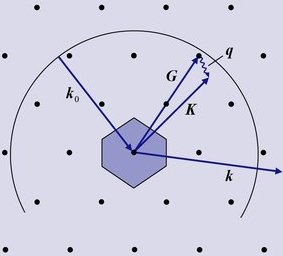
\includegraphics[width=0.6\textwidth]{ewald-kugel}
\centering
\label{fig:ewald-kugel}
\end{figure}
Der Impulsübertrag in dem Bild setzt sich aus dem Anteil $\hbar\bm{G}$ zusammen
, den das Gitter übernimmt und dem Quasiimpuls $\hbar\bm{q}$ des vernichteten
Photons. Der Betrag des Wellenvektors vergrößert sich, und der Wellenvektor
endet außerhalb der Kugel.
\subsection{Spezifische Wärmekapazität}
\begin{equation}
  C_V=\left(\frac{\partial U}{\partial T}\right)_V
\end{equation}
\begin{equation}
  C_P-C_V=\alpha^2_VVTB
\end{equation}
$\alpha_V$ ist der thermische Volumenausdehnungskoeffizient und B das
Kompressionsmodul. Der typische Verlauf der spezifischen Wärme für einen
Festkörper ist in Abbildung \ref{fig:spezifische} zu sehen.
\begin{figure}[h]
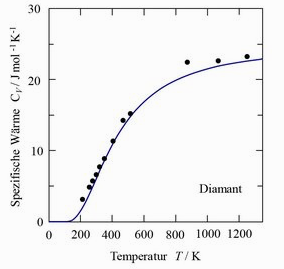
\includegraphics[width=0.6\textwidth]{spezifische}
\centering
\label{fig:spezifische}
\end{figure}

Von tiefen Temperaturen kommend steigt die spezifische Wärme zunächst steil an
und nähert sich dann einem konstanten Wert, der durch das \textbf{Dulong-Petit-
Gesetz} $C_V=3N_Ak_B=3R_m$ gegeben ist. Dieser Verlauf wurde von Einstein
erklärt. Er nahm an, dass die Atome des Festkörpers als ungekoppelte,
harmonische Oszillatoren mit einheitlicher Eigenfrequenz augefasst werden
können. Die Energie der Oszillatoren ist dabei gequantelt. Die spezifische
Wärme muss bei tiefen Temperaturen verschwinden, da die Energie nicht mehr
ausreicht, um die Oszillatoren zu Schwingungen anzuregen. Dies ist das
Einsteinsche Modell der spezifischen Wärme. Nun ist es aber so, dass die Atome
untereinander gekoppelt sind.
\subsubsection{Zustandsdichte der Phononen}
Die endliche Größe eines Festkörpers und somit die endliche Zahl an Atomen
schränkt die Zahl der möglichen Eigenschwingungen durch Randbedingungen ein.
Man erhält periodische Randbedingungen, wenn man einen makroskopischen Kristall
endlicher Größe periodisch fortsetzt. Es entsteht ein unendlich ausgedehnter
Gesamtkristall. Dies führt beispielsweise zu:
\begin{equation}
  e^{i\bm{q}\cdot\bm{r}}=e^{i\bm{q}\cdot\bm{r}}e^{q_xL}
\end{equation}
Die Periodizität ist gewährleistet, wenn gilt:
\begin{equation}
  q_x = \frac{2\pi}{L}m_x
\end{equation}
Für eine beliebige ganze Zahl $m_x$. Weiter gilt die Einschränkung:
\begin{equation}
  -\frac{\mathcal{M}}{2}<m_i\leq\frac{\mathcal{M}}{2}
\end{equation}
Wenn wir den Bewegungszustand der Atome am Rand festsetzen, z.B. als unbeweglich
, erhalten wir feste Ransbedingungen. Diese führen nun, im Gegensatz zu
periodischen Wellen zu stehenden statt laufenden Wellen. Da bei stehenden
Wellen die Periodizität durch die halbe Wellenlänge gegeben ist, gilt nun:
\begin{equation}
  q_x = \frac{\pi}{L}m_x
\end{equation}
und weiter
\begin{equation}
  0<m_i\leq\mathcal{M}
\end{equation}
Da alle erlaubten Wellenvektoren in \textbf{einer} Elementarzelle liegen, ist
ihre Dichte $\rho_q$ im reziproken Raum durch das Verhältnis Anzahl N der
erlaubten Zustände pro Volumen der Elementarzelle des reziproken Gitters
gegeben. Somit folgt:
\begin{equation}
  \rho_q=\frac{\mathcal{N}}{(2\pi)^3/V_Z}=\frac{V}{(2\pi)^3}
\end{equation}
Die Zustandsdichte im reziproken Raum hängt also nur vom Probenvolumen ab. Für
niederdimensionale Systeme gilt:
\begin{equation}
  \begin{align}
    \rho_q^{(1)}&=\frac{L}{2\pi} \\
    \rho_q^{(2)}&=\frac{A}{(2\pi)^2}
  \end{align}
\end{equation}
Nun ermitteln wir die Dichte der Zustände im Frequenzraum $D(\omega)$. Dazu
betrachten wir die Anzahl der Zustände zwischen $S(\omega)$ und $S(\omega+d
\omega)$. In dieser Schale müssen wir alle Zustände aufsummieren.
\begin{equation}
  \mathcal{D}(\omega)d\omega=\rho_q
  \int_{\omega=const}^{\omega+d\omega=const}d^3q
\end{equation}
Wir drücken das Volumenelement durch $d^3q=dq_\perp dS_\omega$ aus. Zum
umformen von $dq_\perp$ benutzen wir die Definition der Gruppengeschwindigkeit.
\begin{equation}
  v_g=\abs{\frac{d\omega}{d\bm{q}}}=\abs{grad_\bm{q}\omega}=
  \abs{\frac{d\omega}{dq_\perp}}
\end{equation}
und somit:
\begin{equation}
  \abs{dq_\perp}=\frac{d\omega}{v_g}
\end{equation}
Für die Zustandsdichte folgt:
\begin{equation}
  \mathcal{D}(\omega)d\omega=\rho_qd(\omega)\int_{w=const}\frac{dS_\omega}
  {\abs{grad_\bm{q}\omega}}=
  \frac{V}{(2\pi)^3}d\omega\int_{w=const}\frac{dS_\omega}{v_g}
\end{equation}
Bei isotropen Festkörpern ist die Fläche konstanter Frequenz im reziproken Raum
die Oberfläche einer Kugel, auf der die Gruppengeschwindigkeit konstant ist. Mit
q als Radius dieser Kugel ergibt sich:
\begin{equation}
  \mathcal{D}(\omega)d\omega=\rho_qd(\omega)\frac{4\pi q^2}{v_g}
  =\frac{V}{2\pi^2}\frac{q^2}{v_g}d\omega
\end{equation}
Die Verteilung wird also stark von der Gruppengeschwindigkeit beeinflusst. Je
flacher die Dispersionsrelation verläuft, umso dichter liegen die Zustände.
Anzumerken bleibt, dass wir bisher nur die Zustandsdichte eines Zweiges
betrachtet haben, am Ende muss zwangsläufig über alle Zweige summiert werden.
\subsubsection{Spezifische Wärme in der Debye-Näherung}
Für alle Wellenvektoren wird die Beziehung $\omega=vq$ vorausgestzt, die
eigentlich nur für große Wellenlängen gilt. Wir benutzen die Näherung des
elastischen Kontinuums bis zu den höchsten Frequenzen. So vereinfacht sich die
Zustandsdichte zu
\begin{equation}
  \mathcal{D}(\omega)d\omega=\frac{V}{2\pi^2}\frac{\omega^2}{v^3}d\omega
\end{equation}
Auf Grund der bergrenzten Zahl an Schwingungszuständen muss eine obere
Abschneidefrequenz $\omega_{max}$ existieren. Diese wird über die Zahl der
erlaubten Schwingungszustände pro Zweig definiert.
\begin{equation}
  N = \int_0^{\omega_{max}}\frac{V}{2\pi^2}\frac{\omega^2}{v^3}d\omega
\end{equation}
Es folgt für die Abschneidefrequenz:
\begin{equation}
  \omega_{max}=v\sqrt[3]{\frac{6\pi^2N}{V}}=\frac{v}{a}\sqrt[3]{6\pi^2}
\end{equation}
wobei wir $\frac{V}{N}=a^3$ benutzen. Berücksichtigen wir alle drei Zweige, so
ergibt sich:
\begin{equation}
  \mathcal{D}(\omega)d\omega=\frac{3V}{2\pi^2}\frac{\omega^2}{v^3_D}d\omega
\end{equation}
mit der Debye-Geschwindigkeit
\begin{equation}
  \frac{3}{v_D^3}=\frac{1}{v_l^3}+\frac{2}{v_t^3}
\end{equation}
Für die innere Energie gilt nun einfach:
\begin{equation}
  U=\int_0^{\omega_D}\hbar\omega\mathcal{D}(\omega)\langle n(\omega,T)\rangle
  d\omega
\end{equation}
wobei für den Bose-Einstein-Faktor gilt:
\begin{equation}
  \langle n(\omega,T)\rangle=\frac{1}{e^{\frac{\hbar\omega}{k_BT}}-1}
\end{equation}
Er gibt bei harmonischen Oszillationen an, wie viele Energieniveaus im
Mittel besetzt sind. In unserem Fall sagt er, wie viele Phononen mit der
Frequenz $\omega$ pro erlaubten Schwingungszustand im Mittel besetzt sind.
Für die innere Energie gilt nun:
\begin{equation}
  U(T)=\frac{9N}{w_D^3}\int_0^{w_D}\frac{\hbar\omega^3}{e^{\frac{\hbar
  \omega}{k_BT}}-1}d\omega
\end{equation}
Nun führen wir die Debye-Temperatur ein:
\begin{equation}
  \begin{align}
    k_B\Theta&=\hbar\omega_D \\
    x&=\frac{\hbar\omega}{k_BT}\\
    x_D&=\frac{\hbar\omega_D}{k_BT}=\frac{\Theta}{T}
  \end{align}
\end{equation}
Damit folgt:
\begin{equation}\label{debye}
  C_V=\left(\frac{\partial U}{\partial T}\right)_V=9Nk_B\left(\frac{T}{\Theta}
  \right)^3\int_0^{x_D}\frac{x^4e^x}{(e^x-1)^2}dx
\end{equation}
Dies ist die Debye-Formel. Für hohe Temperaturen geht $x \to 0$. Das Integral
vereinfacht sich in diesem Fall:
\begin{equation}
  \int_0^{x_D}\frac{x^4e^x}{(e^x-1)^2}dx \approx \int_0^{x_D}\frac{x^4\cdot 1}
  {(1+x-1)^2}dx = \int_0^{x_D}x^2dx=\frac{1}{3}\left(\frac{\Theta}{T}\right)^3
\end{equation}
Setzen wir dies in Gleichung \ref{debye} ein, erhalten wir eine Übereinstimmung
mit dem Dulong-Petit-Gesetz für die molare Wärmekapazität $C_V=3N_Ak_B=3R_m$.
Für tiefe Temperaturen geht die Integrationsgrenze $x_D\to\infty$. Man findet
analytisch für das Integral:
\begin{equation}
  \int_0^\infty\frac{x^4e^x}{(e^x-1)^2}dx=\frac{4\pi^4}{15}
\end{equation}
Damit ergibt sich für die molare Wärme:
\begin{equation}
  C_V=\frac{12\pi^4}{5}Nk_B\left(\frac{\Theta}{T}\right)^3
\end{equation}
Dies ist das $T^3$-Gesetz für die spezifische Wärme von Festkörpern bei tiefen
Temperaturen. Die Debye-Näherung ist gut für tiefe Temperaturen $T<\frac{\Theta}
{100}$ und für hohe Temperaturen $T>\frac{\Theta}{5}$.
\subsubsection{Spezifische Wärme niederdimensionaler Systeme}
Für ein zweidimensionales System mit Zustandsdichte
\begin{equation}
  \mathcal{D}^{(2)}(\omega)=\frac{A}{4\pi^2}\frac{2\pi q}{v_g}=\frac{A}{2\pi}
  \frac{q}{v_g}
\end{equation}
erhalten wir für die Berechnung der spezifischen Wärme im Grenzfall niedriger
Temperaturen
\begin{equation}
  C_V \propto T^2
\end{equation}
\subsection{Wärmetransport in Kristallen}
In dielektrischen Kristallen wird die Wärme durch Gitterstöße, also Phononen
transportiert. Wir unterscheiden zwischen der klassischen Wärmeleitung, bei der
die Phononen durch die Probe diffundieren und der ballistischen Wärmeleitung,
bei der sie ohne größere Wechselwirkung durch die Probe laufen.
\subsubsection{Wärmeleitfähigkeit}
Wenn die Phononen nicht wie in Wärmepulsexperimenten nahezu Stoßfrei die Probe
durchqueren, sondern sich durch Diffusion ausbreiten, so wird der
Energietransport durch den Temperaturgradienten bestimmt.
\begin{equation}
  \bm{j}=-\Lambda grad T
\end{equation}
wobei $\bm{j}$ für die Wärmestromdichte und $\Lambda$ für den Koeffizienten der
Wärmeleitfähigkeit steht. Zur Beschreibung der Wärmeleitung stützen wir uns auf
die Analogie zur kinetischen Gastheorie und betrachten die Phononen als ideales
Gas.
\begin{equation}
  \Lambda=\frac{1}{3}Cvl
\end{equation}
C ist die spezifische Wärme des Gases, v die mittlere Geschwindigkeit der Atome
und l die mittlere freie Weglänge. In dem wir diese Gleichung übernehmen, steht
v nun für die Schallgeschwindigkeit im Kristall und l für die mittlere freie
Weglänge der Phononen. Es treten bei Phononen zwei Streumechanismen auf.
Entweder sie werden aneinander, oder an Defekten gestreut. Die mittleren freien
Weglängen der unterschiedlichen Streumechanismen addieren sich invers.
\subsubsection{Phononenstöße}
Wir machen die inelastischen 3-Phononen-Stöße für den Wärmewiderstand
verantwortlich. Es gilt Energie- und Quasiimpulserhaltung.
\begin{equation}
  \hbar\omega_1\pm\hbar\omega_2=\hbar\omega_3
\end{equation}
\begin{equation}
  \hbar\bm{q}_1\pm\hbar\bm{q}_2=\hbar\bm{q}_3+\hbar\bm{G}
\end{equation}
Je nach Vorzeichen wird beim Stoß ein Phonon erzeugt oder vernichtet. Wie bei
der inelastischen Streeung von Wellen kann ein reziproker Gittervektor $\bm{G}$
 auftreten. Dieser spielt bei der Wärmeleitung eine wichtige Rolle. Wenn er an
einem Streuprozess beteiligt ist, spricht man von einem Umklapp- oder U-Prozess.
Ist er nicht beteiligt, spricht man von einem Normal-oder N-Prozess.
Sind die Wellenvektoren der beteiligten Phononen relativ klein, so läuft der
Prozess innerhalb der ersten Brillouin-Zone ab. Endet der resultierende Vektor
$\bm{q}_3$ außerhalb der ersten Brillouin-Zone, so lässt sich durch Addition
des reziproken Gittervektors $\bm{G}$ ein Vektor $\bm{q}_3'$ finden, der
innerhalb der ersten Brillouin-Zone endet. Beide Prozesse sind in Abbildung
\ref{fig:umklapp} dargestellt.
\begin{figure}[h]
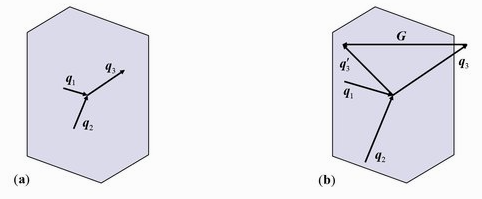
\includegraphics[width=0.6\textwidth]{umklapp}
\centering
\label{fig:umklapp}
\end{figure}
Bei N-Prozessen bleibt die Summer der Quasiimpulse der beteiligten Phononen
erhalten. Da durch die Stöße weder der Impulsfluss noch der damit verknüpfte
Energiefluss beeinflusst wird, tragen diese Stöße nicht zum Wärmewiderstand bei.
Gäbe es nur N-Prozesse, dann würde eine Verteilung heißer Phononen mit einem
Gesamtimpuls $\bm{P}$ ohne Änderung von $\bm{P}$ durch die Probe laufen, die
Wärmeleitfähigkeit währe unendlich groß. Bei Umklappprozessen liegt der
Wellenvektor des resultierenden Phonons außerhalb der 1. Brillouin-Zone. Die
Gruppengeschwindigkeiten der stoßenden Phononen und des resultierenden Phonons
weißen unterschiedliche Vorzeichen auf, die Energie wird in die entgegengesetzte
Richtung transportiert. Bei hohen Temperaturen dominieren Umklappprozesse, da
die Wellenvektoren der meisten Phononen am Rand der Brillouin-Zone liegen und
somit fast jeder Stoß zu einem Umklappprozess führt. Bei hohen Temperaturen
$T>\Theta$ ist $l^{-1}\propto \omega_DT$. Die spezifische Wärme ist näherungsweise
konstant, und so gilt:
\begin{equation}
  \Lambda \propto\frac{1}{T}
\end{equation}
Für mittlere Temperaturen $T\leq\Theta$ gilt dagegen:
\begin{equation}
  \Lambda\propto e^{\frac{\Theta}{2T}}
\end{equation}
Bei tiefen Temperaturen sterben Umklapp-Prozesse aus. Da die Wärmeleitfähigkeit
aber wieder abnimmt, muss es einen weiteren Effekt geben, der den Wärmetransport
begrenzt. Dies ist die Streuung an der Oberfläche des Körpers. Der Gesamtimpuls
ändert sich ähnlich wie bei Umklappprozessen, und wir setzten den
Probedurchmesser $d\approx l$.
\begin{equation}
  \Lambda=C_Vvd\propto T^3d
\end{equation}
Den Bereich, in dem die Wärmeleitfähigkeit von dem Probendurchmesser abhängt,
bezeichnet man als Casimir-Bereich. Die mittlere freie Weglänge hängt hier auch
von der Oberflächenbeschaffenheit ab. Bei gut polierten Oberflächen tritt
Spiegelung auf, wodurch sich der Impuls parallel zur Oberfläche nicht ändert.
Die mittlere freie Weglänge wird somit größer als die Propendicke.
\section{Elektronen im Festkörper}
\subsection{Freies Elektronengas}
In manchen Metallen lassen sich die elektronischen Eigenschaften gut auf das
Verhalten freier Elektronen zurückführen. Die Elektronen bewegen sich in einem
konstanten Potential, eine Barriere ist nur am Probenrand vorhanden. Ein
Elektron mit der Energie $E_F$ ist an den Festkörper gebunden, solange $E_F<W$
ist, wobei W die Potentialtiefe ist. Die Austrittsarbeit ist definiert als
$Phi=(W-E_F)$. Von einem Elektronengas oder \textbf{Fermi-Gas} spricht man, wenn
sich die Leitungselektronen in guter Näherung wie ein klassisches Gas verhalten.
Allerdings sind die Elektronen dem Pauli-Prinzip unterworfen. Diese Näherung
geht auf A. Sommerfeld zurück. Nun haben wir aber gesehen, dass Valenzelektronen
die Atomrümpfe meiden. Diese Tatsache wird berücksichtigt, indem man ein
Pseudopotential einführt. Dieses Berücksichtigt, dass für Valenzelektronen die
effektive Variation des Potentials wesentlich schwächer ist, als man zunächst
vermutet. Die Leitungselektronen sehen nicht das nackte Coulomb-Potential,
sondern das viel schwächere Pseudopotential. Diese starke Vereinfachung ist bei
den Alkali-oder einfachen Metallen wie Kupfer, Silber, Gold sehr gut. Dort sind
neben den delokalisierten freien s-Elektronen nur Elektronen in abgeschlossenen
Schalen vorhanden. Dagegen ist die Annahme quasi-freier Elektronen bei vielen
Übergangsmetallen nur bedingt erfüllt. Bei diesen Metallen tragen neben den
s-Elektronen auch noch d- und/oder f-Elektronen in teilgefüllten Schalen bei.
\subsubsection{Zustandsdichte}
Wir setzen als Lösung der Schrödingergleichung für die Elektronen als
Wellenfunktion eine ebene Welle an:
\begin{equation}
  \psi(\bm{r})=\frac{1}{\sqrt{V}}e^{i\bm{k}{r}}
\end{equation}
Für die Energieeigenwerte E freier Elektronen gilt:
\begin{equation}
  E=\frac{\hbar^2k^2}{2m}
\end{equation}
Wir benutzen auch für die Elektronenwellenfunktion periodische Randbedingungen,
so dass für die Wellenvektoren folgt:
\begin{equation}
  k_i=\frac{2\pi}{L}m_i
\end{equation}
Die Wellenvektoren sind wie bei den Phononen gleichmäßig im Impulsraum verteilt
und haben die Dichte $\rho_k'=\frac{V}{(2\pi)^3}$. Nach dem Pauli-Prinzip kann
jeder Zustand mit zwei Elektronen mit unterschiedlichen Spin-Richtungen besetzt
werden, so dass für die Zustandsdichte im Impulsraum gilt:
\begin{equation}
  \rho_k=\frac{2V}{(2\pi^3)}
\end{equation}
Die Zustandsdichte D(E) im Energieraum
\begin{equation}
  \mathcal{D}(E)dE=\rho_k\int_E^{E+dE}d^3k=\frac{\rho_k}{\hbar}dE\int_{E=const}
  \frac{dS_E}{v_g}
\end{equation}
Die Gruppengeschwindigkeit $v_g=\frac{\partial E}{\partial (\hbar k)}=\frac
{\hbar k}{m}$ hängt beim Elektronengas nicht von der Richtung ab. Damit hat die
Fläche konstanter Energie die Gestalt einer Kugel und das Oberflächenintegral
ergibt $\int dS_E=4\pi k^2$. Für die Zustandsdichte folgt somit:
\begin{equation}
  \mathcal{D}(E)=\frac{2V}{(2\pi^3)\hbar}\frac{m}{\hbar k}4\pi k^2=
  \frac{V}{2\pi^2}\left( \frac{2m}{\hbar^2} \right)^{\frac{3}{2}}\sqrt{E}
\end{equation}
und für die elektronische Zustandsdichte pro Volumen $D(E)=\frac{\mathcal{D}
(E)}{V}$:
\begin{equation}
  D(E)=\frac{1}{2\pi^2}\left( \frac{2m}{\hbar^2}\right)^{\frac{3}{2}}\sqrt{E}
\end{equation}
Obwohl die Dichte von Zuständen von Elektronen und Phononen im reziproken
Raum gleich ist, unterscheiden sich ihre Zustandsdichten aufgrund der
unterschiedlichen Dispersionsrelationen.
\noindent \paragraph{Niedrigdimensionale Elektronensysteme}
Wir untersuchen Energiespektrum E(k) und Zustandsdichte D(E) für
niederdimensionale Proben. Für die Zustandsdichte gilt:
\begin{equation}
  \rho_k^{(\alpha)}=2\left(\frac{L}{2\pi}\right)^{\alpha}
\end{equation}
Die Integration über die Oberfläche reduziert sich im zweidimensionalen auf ein
Linienintegral, das im isotropen Raum den Wert $2\pi k$ ergibt. Es folgt:
\begin{equation}
  D^{(2)}(E)=\frac{\rho_k^{(2)}}{A\hbar}\frac{2\pi k}{v_g}=\frac{m}{\pi\hbar^2}
\end{equation}
Die Zustandsdichte eines zweidimensionalen Elektronengases ist energieunabhänig,
also konstant.
\subsubsection{Fermi-Energie}
In einem Ensemble von Teilchen mit halbzahligem Spin ist das Pauli-Prinzip
wirksam. Das bedeutet, dass die Besetzung der Zustände durch die Fermi-Dirac-
Statistik bestimmt wird. Die Besetzungswahrscheinlichkeit wird daher durch die
Fermi-Verteilung
\begin{equation}
  f(E)=\frac{1}{e^{\frac{(E-\mu)}{k_BT}}+1}
\end{equation}
ausgedrückt. Das chemische Potential $\mu$, stellt den Zusammenhang zwischen
der freien Energie F und der Teilchenzahl N her:
\begin{equation}
  \mu=\left(\frac{\partial F}{\partial N}\right)_{T,V}
\end{equation}
Bei $T=0$ sind also alle Zustände mit $E<\mu$ besetzt, wobei jeweils zwei
Elektronen pro Zustand erlaubt sind. Die Energie, bis zu der die Zustände
lückenlos gefüllt sind, bezeichnet man als Fermi-Energie. Da das chemische
Potential die kleinste Energie angibt, die man braucht, um ein zusätzliches
Elektron in das Fermi-Gas einzubringen, und dies bei $T=0$ nur bei der Fermi-
Energie geschehen kann, gilt $E_F=\mu(T=0)$. Die Fermi-Energie ist durch die
Elektronendichte $n=\frac{N}{V}$ festgelegt. Integriert man über alle besetzten
Zustände, so erhält man gerade die Teilchenzahl:
\begin{equation}
  n=\frac{N}{V}=\int_0^\infty D(E)f(E,T=0)dE=\int_0^{E_F}D(E)dE=\frac{1}{2\pi^2}
  \left( \frac{2m}{\hbar^2}\right)^{\frac{3}{2}}\frac{2E_F^{\frac{3}{2}}}{3}
\end{equation}
Lösen wir diese Gleichung nach $E_F$ auf, so sehen wir, dass die Fermi-Energie
nur durch die Massen und Konzentration der Elektronen bestimmt ist:
\begin{equation}
  E_F=\frac{\hbar^2}{2m}(3\pi^2n)^{\frac{2}{3}}
\end{equation}
Weiter definieren wir:
\begin{equation}
  k_F=(3\pi^2n)^{\frac{2}{3}}\quad \text{Fermi-Wellenvektor}
\end{equation}
\begin{equation}
  v_F=\frac{\hbar}{}(3\pi^2n)^{\frac{2}{3}}\quad \text{Fermi-Geschwindigkeit}
\end{equation}
\begin{equation}
  T_F=\frac{E_F}{k_B}\quad \text{Fermi-Temperatur}
\end{equation}
Für die Zustandsdichte $D(E_F)$ an der Fermi-Kante gilt:
\begin{equation}
  D(E_F)=\frac{3}{2}\frac{n}{E_F}
\end{equation}
Bei endlicher Temperatur werden unterhalb der Fermi-Kante Zustände frei und
oberhalb von $E_F$ Zustände besetzt, die am absoluten Nullpunkt unbesetzt waren.
Es erfolgt eine 'Aufweichung' der Fermi-Kante mit einer Breite von etwa $2k_BT$.
Es wird also nur ein Bruchteil der Elektronen der Größenordnung $\frac{T}{T_F}$
thermisch angeregt. Der Wert des chemischen Potentials ist durch die Bedingung
$f(E,T)=\frac{1}{2}$ festgelegt und nimmt mit steigender Temperatur leicht ab.
Solange $T\ll T_F$ sit, lässt sich die Temperaturabhängigkeit durch die
Sommerfeld-Entwicklung
\begin{equation}
  \mu(T)\approx E_F\left[1-\frac{\pi^2}{12}\left(\frac{T}{T_F}\right)^2\right]
\end{equation}
ausdrücken. In unserem Modell freier Elektronen besitzt der Betrag des Fermi-
Wellenvektors einen festen richtungsunabhängigen Wert. Die Elektronen sind bei
$T=0$ im Impuls-Raum innerhalb der \textbf{Fermi-Kugel} lokalisiert, deren
Radius durch die Dichte der Elektronen bestimmt wird. Die Oberfläche der Kugel
bezeichnet man als Fermi-Fläche.
\subsection{Spezifische Wärme}
Wir berechnen nun die innere Energie des Fermi-Gases, um damit die spezifische
Wärme der Metallelektronen herzuleiten. Am abosluten Nullpunkt finden wir für
die innere Energie pro Volumen $u_0=\frac{U}{V}$ den Ausdruck:
\begin{equation}
  u_0=\int_0^\infty ED(E)f(E,T=0)dE=\int_0^{E_F}ED(E)dE=\frac{3n}{5}E_F=
  \frac{3n}{5}k_BT_F
\end{equation}
Auf Grund der hohen Fermi-Temperatur ist selbst bei $T=0$ die innere Energie der
Elektronen sehr viel größer als die eines klassichen Gases. Für die spezifische
Wärme entscheidend ist aber der temperaturabhängige Anteil. Dieser entspricht
dem Bruchteil der Elektronen, die die thermische Energie $k_BT$ aufnehmen kann,
grob durch $\frac{T}{T_F}$ gegeben. Somit ist $\delta u(T)=u(T)-u_0=nk_BT\cdot
\frac{T}{T_F}$ und es folgt:
\begin{equation}
  c_V^{el}=\left(\frac{\partial u}{\partial T}\right)_V\approx\frac{2nk_BT}{T_F}
\end{equation}
Verglichen mit einem klassischen Gas tritt also eine deutliche Reduktion der
spezifischen Wärme um den Faktor $\frac{T}{T_F}$ auf. Um genauer zu Rechnen
müssten wir das Fermi-Dirac-Integral
\begin{equation}
  u=\int_0^\infty ED(E)f(E,T)dE
\end{equation}
lösen, was analytisch nicht möglich ist. Eine Näherungslösung ergibt
\begin{equation}
  c_V^{el}\approx\frac{\pi^2T}{3T_F}\frac{3nk_B}{2}=\gamma T
\end{equation}
Der Faktor $\frac{\pi^2T}{3T_F}$ gibt die Reduktion gegenüber der spezifischen
Wärme eines klassischen Gases an. $\gamma$ wird auch als Sommerfeld-Konstante
bezeichnet und ist durch die Dichte und Masse der Elektronen festgelegt. Die
\textbf{gesamte spezifische Wärme} pro Volumen eines Metalls setzt sich nun aus
dem Beitrag der Elektronen und des Gitters zusammen:
\begin{equation}
  c_V^{ges}=\gamma T + \begin{cases}
  3n_Ak_B & \text{für } T>\Theta \\
  \beta T^3 & \text{für } T\ll\Theta
  \end{cases}
\end{equation}
Bei hohen Temperaturen dominiert der Beitrag des Gitter, der durch das Dulong-
Petit-Gesetzt genähert wird. Bei tiefen Temperaturen trägt das Gitter den Term
$\beta T^3$ zur spezifischen Wärme bei. Bei ungefähr 4K sind die Beiträge von
Elektronen und Gitter gleich groß. Um die beiden Beiträge zu trennen, trägt man
am Besten $\frac{c_V}{T}$ als Funktion von $T^2$ auf. Der Wert von $\gamma$
lässt sich nun als Achsenabschnitt ablesen, aus der Steigung ergibt sich
$\beta$. Dies ist in Abbildung \ref{fig:spezifische2} sichtbar.
\begin{figure}[h]
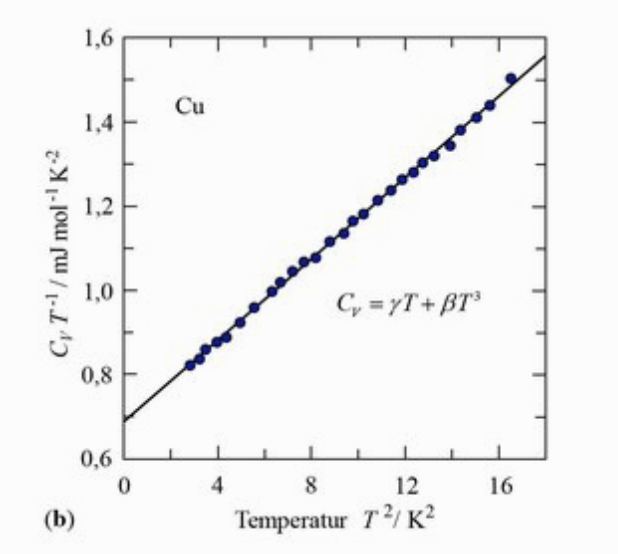
\includegraphics[width=0.6\textwidth]{spezifische2}
\centering
\label{fig:spezifische2}
\end{figure}
Diese Näherung ist bei einfachen Metallen sehr gut, doch bei Ag, Au und Pb
ergeben sich teils größere Abweichungen. $\gamma$ ist proportional zur Masse und
zur Konzentration der Elektronen. Der Grund für die Abweichung ist, dass
Elektronen als freie Teilchen behandelt wurden. In Wirklichkeit spüren die
Leitunselektronen das periodische Potential des Gitters. Dies wird durch die
Einführung einer thermischen effektiven Masse $m^*$ berücksichtigt. Diese ist
durch
\begin{equation}
  \frac{m_th^*}{m}=\frac{\gamma_{exp}}{\gamma_{theo}}
\end{equation}
definiert.
\subsection{Elektronen im periodischen Potential}
Das Modell freier Elektronen besticht durch seine Einfachheit, hat aber auch
physikalische Grenzen. So würde man erwarten, dass immer wenn Elektronenschalen
eines Elements nicht vollkomnmen aufgefüllt sind, sich die Elektronen dieser
Schalen relativ frei bewegen können, und das Element einen metallischen
Character besitzt. Dies ist aber offensichtlich bei Diamant nicht der Fall, der
ein guter Isolator sit, obwohl die äußere Schale nur halb gefüllt ist. Bei
Natrium finden wir erwartungsgemäß ein freies Elektron pro Atom. Bei Beryllium
würden wir nun zwei freie Elektronen pro Atom erwarten, finden jedoch 0.2
positive Ladungsträger pro Atom. Wir müssen berücksichtigen, dass dich die
Elektronen im periodischen Potential bewegen.
\subsubsection{Bloch-Funktion}
Wir beschreiben das Verhalten der Elektronen im periodischen Gitterpotential in
der Einelektron-Näherung. Das Potential, das die Translationssymmetrie des
Gitters besitzt, lässt sich wie die Streudichte in eine Fourier-Reihe nach
reziproken Gittervektoren $\bm{G}$ entwickeln.
\begin{equation}
  \tilde{V}(\bm{r})=\sum_{\bm{G}}\tilde{V}_{\bm{G}}e^{i\bm{G}\cdot\bm{r}}
\end{equation}
Nun wählen wir für die Wellenfuktion des betrachteten Elektrons den Ansatz:
\begin{equation}
  \psi_{\bm{r}}=\sum_{\bm{k}}e^{i\bm{k}\cdot\bm{r}}
\end{equation}
wobei die Koeffizienten $c_{\bm{k}}$ im Laufe der Rechnung bestimmt werden.
Nun setzten wir die Potenzreihenentwicklung und den Ansatz für die
Wellenfunktion in die Schrödingergleichung ein. Wir erhalten das Ergebnis:
\begin{equation}
  \left(\frac{\hbar^2k^2}{2m}-E\right)c_{\bm{k}}+\sum_{\bm{G}}
  \tilde{G}_{\bm{G}}c_{\bm{k}-\bm{G}}=0
\end{equation}
Dieser Satz Gleichungen ist die Darstellung der Schrödinger-Gleichung im k-Raum
für ein Elektron, das sich in einem periodischen Potential bewegt. Für jeden
Wellenvektor $\bm{k}$ gibt es ein Gleichungssystem mit der Wellenfunktion
$\psi_{\bm{k}}(\bm{r})$ und dem dazugehörigen Eigenwert $E_{\bm{k}}$ als
Lösung. Es treten nur noch Entwicklungskoeffizienten auf, die sich um reziproke
Gittervektoren unterscheiden. Dies bedeutet, dass sich $\psi_{\bm{k}}(\bm{r})$
aus ebenen Wellen zusammensetzt, deren Wellenvektoren $\bm{k}$ sich ebenfalls
um reziproke Gittervektoren $\bm{G}$ unterscheiden. Die Entwicklung vereinfacht
sich zu:
\begin{equation}
  \psi_{\bm{k}}(\bm{r})=\sum_{\bm{G}}c_{\bm{k}-\bm{G}}
  e^{i(\bm{k}-\bm{G})\cdot\bm{r}}
\end{equation}
Dies bringen wir nun in die Form:
\begin{equation}
  \psi_{\bm{k}}(\bm{r})=\left(\sum_{\bm{G}}c_{\bm{k}-\bm{G}}
  e^{-i\bm{G}\cdot\bm{r}}\right)e^{i\bm{k}\cdot\bm{r}}
\end{equation}
Der Ausdruck in Klammern ist die Fourier-Entwicklung einer gitterperiodischen
Funktion. Die Lösungen der Schrödinger-Gleichung für ein periodisches Potential
sind also ebene Wellen, multipliziert mit einem gitterperiodischen
Modulationsfaktor, den wir $u_{\bm{k}}(\bm{r})$ nennen.
Die Wellenfunktion können wir nun durch die Bloch-Funktion
\begin{equation}
  \psi_{\bm{k}}(\bm{r})=u_{\bm{k}}(\bm{r})e^{i\bm{k}\cdot\bm{r}}
\end{equation}
ausdrücken, wobei die Gitterperiodizität in der Beziehung
\begin{equation}
  u_{\bm{k}}(\bm{r})=u_{\bm{k}}(\bm{r}+\bm{R})
\end{equation}
steckt. Die letzten beiden Gleichungen sind ein Spezialfall eines Theorems von
F.Bloch. Es besagt, dass für jede beliebige Wellenfunktion, die die Schrödinger-
Gleichung erfüllt, ein derartiger Wellenvektor $\bm{k}$ existiert, dass die
Translations um einen Gittervektor $\bm{R}$ gleichwertig ist mit der
Multiplikation um einen Phasenfaktor $e^{i\bm{k}\cdot\bm{R}}$.
\subsubsection{Quasi-freie Elektronen}
Wir nehmen zunächst an, dass die Amplitude des periodischen Potential so klein
ist, dass wir $\tilde{V}_{\bm{G}}\approx 0$ setzen dürfen. Die Symmetrie des
Gitters soll aber weiterhin periodische Lösungen erzwingen. Man spricht von
einem leeren Gitter. Es folgt aus der Periodizität der Eigenwerte:
\begin{equation}
  E_{\bm{K}}=\frac{\hbar^2k^2}{2m}=E_{\bm{k}+\bm{G}}=\frac{\hbar^2}{2m}
  \abs{\bm{k}+\bm{G}}^2
\end{equation}
Es handelt sich um Parabeln, die im k-Raum um $\bm{G}$ gegeneinander verschoben
sind. Betrachten wir ein eindimensionales leeres Gitter mit der Gitterkonstanten
a. Die reziproken Gittervektoren sind durch Vielfache von $g=\frac{2\pi}{a}$
gegeben. Bei der Reduktion auf die 1. Brillouin-Zone verscheibt man die Teile
der Parabeln, die außerhalb der 1. Brillouin-Zone liegen, um einen reziproken
Gittervektor, dass die innerhalb der ersten Zone liegen:
\begin{figure}[h]
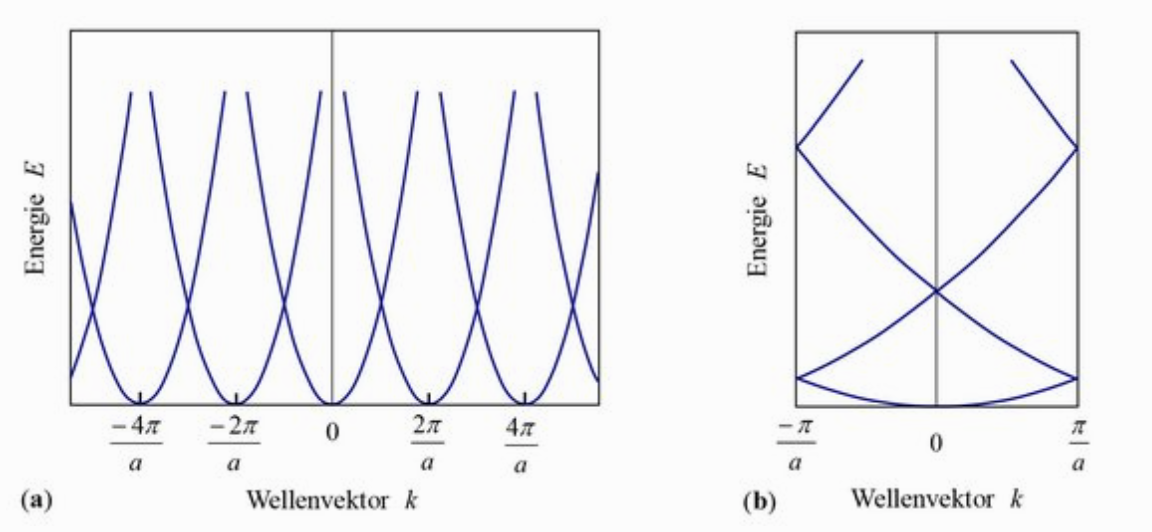
\includegraphics[width=0.6\textwidth]{bloch}
\centering
\label{fig:bloch}
\end{figure}
\subsection{Energiebänder}
\section{Elektronische Transporteigenschaften}
\subsubsection{Elektronen als Wellenpakete}
Inwieweit sind die klassischen Gleichungen wie das 2. Newtonsche Gesetz auf
Elektronen anwendbar, wenn die Unschärferelation erfüllt sein muss?
Wir beschreiben die zeitliche Entwicklung des Ortsvektors $\bm{r}$ und des
Wellenvektors $\bm{k}$ eines Elektrons als Wellenpaket in Gegenwart eines
äußeren elektrischen oder magnetischen Feldes $\bm{\varepsilon}$ bzw.
$\bm{B}$. Die Geschwindigkeit des Wellenpaketes ist durch die
Gruppengeschwindigkeit aus der Disperdionsrelation gegeben:
\begin{equation}
  \frac{d\bm{r}}{dt}=\bm{v}_n(\bm{k})=\frac{1}{\hbar}\nabla_{\bm{k}}E_n(\bm{k})
  =\frac{1}{\hbar}\frac{\partial E_n(\bm{k})}{\partial\bm{k}}
\end{equation}
Hier steht n für den Index des betrachteten Bandes. Für freie Elektronen mit der
parabelförmigen Dispersionsrelation $E=\frac{\hbar^2\bm{k}^2}{2m}$ ergibt sich
die Gruppengeschwindigkeit $\bm{v}_g=\frac{\hbar\bm{k}}{m}$. Wirkt auf ein
Elektron die Kraft $\bm{F}$, so ändert sich sein Wellenvektor und damit der
Quasiimpuls $\hbar\bm{k}$ gemäß
\begin{equation}
  \hbar\frac{d\bm{k}}{dt}=\bm{F}=-e\left[\mathcal{E}(\bm{r},t)+\bm{v}_n(\bm{k})
  \times\bm{B}(\bm{r},t)\right]
\end{equation}
Dies ist die semiklassische \textbf{Bewegungsgleichung}. Wir setzen nun voraus,
dass die angelegten Felder nicht so groß sind, dass Interband-Übergägne
auftreten und sich der Bandindex n ändert. Wenn bei sehr hohen Feldstärken
Übergänge zwischen den Bändern stattfinden, so spricht man vom elektrischen
bzw. magnetischen Durchbruch. Für die Ableitung der Gruppengeschwindigkeit
folgt:
\begin{equation}
  \frac{d\bm{v}}{dt}=\frac{1}{\hbar}\frac{d}{dt}\left(\frac{\partial E(\bm{k})}
  {\partial\bm{k}}\right)=\frac{1}{\hbar}\frac{\partial^2E(\bm{k})}
  {\partial\bm{k}\partial\bm{k}}\frac{\partial\bm{k}}{dt}=
  \frac{1}{\hbar^2}\frac{\partial^2E(\bm{k})}
  {\partial\bm{k}\partial\bm{k}}\bm{F}
\end{equation}
Somit erhalten wir für die kartesischen Komponenten $v_i$:
\begin{equation}
  \frac{dv_i}{dt}=\frac{1}{\hbar^2}\sum_{j=1}^{3}\frac{\partial^2E(\bm{k})}
  {\partial k_i\partial k_j}F_j=\sum_{j=1}^{3}\left(\frac{1}{m^*}\right)_{ij}F_j
\end{equation}
mit
\begin{equation}
  \left(\frac{1}{m^*}\right)_{ij}=\frac{1}{\hbar^2}\frac{\partial^2E(\bm{k})}
  {\partial k_i\partial k_j}
\end{equation}
Mit Hilfe des Tensors der effektiven Masse wird die Verbindung zur klassischen
Bewegungsgleichung $\bm{F}=m\dot{\bm{v}}$ hergestellt. Die reziproke effektive
Masse ist durch die Krümmung der Energiefläche bestimmt. In ihr ist die
Wechselwirkung der Elektronen mit den Atomrümpfen versteckt. Man spricht auch
von der dynamischen Masse. Dieses Konzept wird als effektive Massennäherung
bezeichnet. Für den Impuls folgt nun:
\begin{equation}
  \hbar\bm{k}=[ \bm{m}^*] v
\end{equation}
Wirkt auf ein freies Elektron eine Kraft, so wird es in Kraftrichtung
beschleunigt. Bei den Kristallelektronen erfolgt die Beschleunigung nicht
notwendigerweise in Kraftrichtung, der Betrag der Beschleunigung hängt
zusätzlich von der Wellenzahl ab. Die Tensoren der reziproken effektiven Masse
bzw. der effektiven Masse $\left(\frac{1}{m^*}\right)_{ij}$ und $m^*_{ij}$ sind
symmetrisch. Sie lassen sich daher auf die Hauptachsen transformieren. In
isotropen Festkörpern sind alle Komponenten gleich groß, die effektive Masse ist
dann ein Skalar. Die effektive Masse ist positiv in den Bandminima und negativ
in den Maxima. Die Energieabhängigkeit der effektiven Elektronenmasse hat
überraschende Folgerungen. Legt man an einen idealen Kristall ein elektrisches
Gleichfeld $\bm{\varepsilon}$ and, so wirkt auf die Elektronen eine konstante
Kraft $\bm{F}=-e\bm{\varepsilon}$. Diese bewirkt eine gleichmäßige Bewegung
der Elektronen im $\bm{k}$-Raum. Da sich die Wellenfunktion und der
Energieeigenwert eines Kristallelektrons periodisch wiederholen, resultiert
daraus im realen Taum eine periodische Geschwindigkeitsänderung. Damit verbunden
ist eine oszillatorische Bewegung der Elektronen. Im Idealfall stoßfreier
Elektronbewegung gibt es also bei einem unendlich ausgedehnten Kristall keine
Gleichstromleitfähigkeit. In einem perfekten Kristall würden Elektronen nur noch
\textbf{Bloch-Oszillationen} ausführen. Anschaulich stellt man sich vor, dass
Elektronen an der Grenze der Brillouin-Zone eine Bragg-Reflexion erfahren und
sich ihre Bewegungsrichtung umkehrt. Die Elektronen bwegen sich beim Anliegen
eines elektrischen Feldes im $\bm{k}$-Raum mit konstanter Geschwindigkeit
\begin{equation}
  \abs{\bm{v}}=\frac{e\mathcal{E}}{\hbar}
\end{equation}
durch die Brillouin-Zone mit Ausdehnung $\frac{2\pi}{a}$. Für die
Schwingungsdauer $T_B$ folgt:
\begin{equation}
  T_B=\frac{\frac{2\pi}{a}}{\frac{e\mathcal{E}}{\hbar}}=\frac{h}{ae\mathcal{E}}
\end{equation}
\subsection{Elektronenbewegung in Bändern}
Auch wenn die Bloch-Oszillationen nicht direkt in Erscheinung treten, so hat das
Verhalten der Elektronen im periodischen Potential dennoch erhebliche
Konsequenzen für eine Reihe von Eigenschaften, insbesondere den Stromtransport.
Der Beitrag der einzelnen Elektronen zur Stromdichte $\bm{j}$ hängt von ihrer
Geschwindigkeit ab. Diese wiederum wird durch ihren Wellenvektor bestimmt.
\begin{equation}
  \bm{j}=-\frac{e}{V}\sum_\bm{k}}\bm{v}(\bm{k})
\end{equation}
Nun gehen wir von der Summe $\sum_{\bm{k}}$ zum Integral $\int\rho_kd^3k$ über.
Die Dichte der erlaubten Zustände im Impulsraum $\rho_k=\frac{2V}{(2\pi)^3}$
haben wir bereits hergeleitet. Nur besetzte Zustände tragen zum Ladungstransport
bei.
\begin{equation}
  \bm{j}=-\frac{e}{4\pi^3}\int\bm{v}(\bm{k})f(E,T)d^3k
\end{equation}
Wir betrachten den Stromfluss am absoluten Nullpunkt. Dort ist die Fermi-Dirac-
Verteilung eine Stufenfunktion, die besetzte von unbesetzten Zuständen trennt.
\begin{equation}
  \bm{j}=-\frac{e}{4\pi^3}\int_{\text{besetzt}}\bm{v}(\bm{k})d^3k=
  -\frac{e}{4\pi^3\hbar}\int_{\text{besetzt}}\nabla_kE(\bm{k})d^3k
\end{equation}
Ohne äußeres Feld verschwindet der Stromfluss. Da das reziproke Gitter die
Punktsymmetrie des realen Gitters besitzt, gilt in diesem Fall $E(\bm{k})=
E(-\bm{k})$. Damit folgt für die Geschwindigkeit eines Elektrons mit dem
Wellenvektor $-\bm{k}$_:
\begin{equation}
  \bm{v}(-\bm{k})=\frac{1}{\hbar}\nabla_{-k}E(-\bm{k})=-\frac{1}{\hbar}\nabla_k
  E(\bm{k})=-\bm{b}(\bm{k})
\end{equation}
Elektronen mit entgegengesetzten Wellenvektoren laufen in entgegengesetzte
Richtungen. Da ohne Geld für jedes Elektron mit Wellenvektor $+\bm{k}$ ein
Elektron mit Wellenvektor $-\bm{k}$ zu finden ist, existiert für jedes Elektron
mit Geschwindigkeit $\bm{v}(\bm{k})$ ein Elektron mit Geschwindigkeit
$-\bm{v}(\bm{k})$. Das Integral nimmt daher den Wert null an. Legt man ein
elektrisches Feld an, so ändert sich bei einem vollbesetzten Band nichts an der
Argumentation.
\subsection{Transporteigenschaften}
Das Drude-Modell beruht auf der Annahmen, dass sich die Bewegung der Elektronen
mit Hilfe der kinetischen Gastheorie beschreiben lässt. Die Elektronen werden
wie freie Teilchen behandelt, die sich mit der thermischen Geschwindigkeit
$\bm{v}_{th}$ bewegen und ständig mit den Atomrümpfen stoßen. Es gibt zwei
wichtige Größen, die Driftgeschwindigkeit $\bm{v}_d$ und die mittlere Stoß- und
Relayationszeit $\tau$, die beide in die klassische Bewegungsgleichung für das
Elektron eingehen:
\begin{equation}
  m\frac{d\bm{v}}{dt}=-e\mathcal{E}-m\frac{\bm{v}_d}{\tau}
\end{equation}
Der Term $m\frac{\bm{v}_d}{\tau}$ hat die Form einer Reibungskraft und
berücksichtigt die hemmende Wirkung durch Stöße. Die Driftgeschwindigkeit
$\bm{v}_d=(\bm{v}-\bm{v}_{th})$ spiegelt die vom Feld bewirkte zusätzliche
Geschwindigkeit wider. Die Relaxationszeit $\tau$ sit die Zeit, mit der
$\bm{v}_d$ nach dem Abschalten des Feldes exponentiell dem Wert $\bm{v}_d=0$
entgegen strebt. Im stationären Fall ist $\dot{\bm{v}}=0$ und die
Driftgeschwindigkeit nimmt den Wert
\begin{equation}
  \bm{v}_d=-\frac{e\tau}{m}\bm{\mathcal{E}}=-\mu\bm{\mathcal{E}}
\end{equation}
an. $\mu$ ist dabei die Beweglichkeit. Ist $n$ die Dichte der Elektronen, so
folgt für die Stromdichte:
\begin{equation}
  \bm{j}=-en\bm{v}_d=\frac{ne^2\tau}{m}\bm{\mathcal{E}}=ne\mu\bm{\mathcal{E}}
\end{equation}
und damit für die elektrische Leitfähigkeit
\begin{equation}
  \sigma=\frac{j}{\mathcal{E}}=\frac{ne^2\tau}{m}=ne\mu
\end{equation}
\subsubsection{Elektron-Phonon-Streuung}
Im Gegensatz zur Streuung an Defekten ist die Elektron-Phonon-Streuung
inelastisch. Da $E_F\gg\hbar\omega_D$ ist, wird die Elektronenergie durch die
Erzeugung oder Vernichtung eines Phonons kaum verändert. Für die Wellenzahl der
Elektronen gilt daher in guter Näherung $\abs{\bm{k}}\approx\abs{\bm{k}'}$.
Also können hier nur Elektronen in naher Umgebung der Fermi-Flächen am
Stoßprozess teilnehmen.
Für den Wellenvektor gilt der Erhaltungssatz
\begin{equation}
  \bm{k}=\bm{k}'\pm\bm{q}+\bm{G}
\end{equation}
wobei $\bm{G}$ ein reziproker Gittervektor ist. Das Vorzeichen von $\bm{q}$
hängt davon ab, ob ein Phonon erzeugt oder vernichtet wird. Wie bei der
Phonon-Phonon-Streuung können auch hier zwei Prozesse unterschieden werden:
der Normalprozess ohne Beteiligung eines reziproken Gittervektors und der
Umklapp-Prozess, bei dem $\bm{G}\neq0$ ist. \textbf{Normalprozesse} wirken sich
auf die elektrische Leitfähigkeit je nach Probentemperatur unterschiedlich
stark aus. Wie in Abbildung \ref{fig:streuung} zu sehen, hängt der mittlere
Streuwinkel $\theta$ der Elektronen von der Temperatur ab, da der mittlere
Impulsübertrag von der Wellenzahl und damit von der Frequenz der dominanten
Phononen bestimmt wird. Bei tiefen Temperaturen bewirkt jeder Streuprozess nur
eine relativ kleine Winkeländerung. Daher sind viele Streuereignisse nötig, bis
ein Elektron von der Vorderseite der Fermi-Kugel die Rückseite erreicht. Die
Zeit, bis der Übergang zur Rückseite abgeschlossen ist, hat somit die Bedeutung
einer effektiven mittleren Stoßzeit. Diese Zeit ist relativ lang, da bei tiefen
Temperaturen nur Phononen mit kleiner Wellenzahl beteiligt sind. Mit zunehmender
Temperatur wächst der Streuwinkel an und die Normalprozesse werden immer
effektiver, bis schließlich ein Stoß ausreicht. Zu einem
\textbf{Umklapp-Prozess} kommt es, wenn der Wellenvektor des Elektrons nach dem
Stoß mit dem Phonon, außerhalb der 1. Brillouin-Zone liegt. Hierfür ist ein
Mindestimpuls des beteiligten Phonons erforderlich. Da aber die Fermi-Fläche
in vielen Fällen in der Nähe der Brillouin-Zonengrenze liegt, kann der Impuls
bzw. die Energie des benötigten Phonons, abhängig von der Form der Fermi-Fläche
relativ klein sein. Umklapp-Prozesse können bei einer entsprechenden Form der
Fermi-Fläche zu großen Richtungsänderungen führen, wenn der Impuls des
beteiligten Phonons so klein ist, dass Normalprozesse nur kleine
Winkeländerungen bewirken würden. Diese Prozesse sind deshalb ein besonders
effektiver Mechanismus zur Einstellung des stationären Gleichgewichts beim
elektrischen Ladungstransport.
\begin{figure}[h]
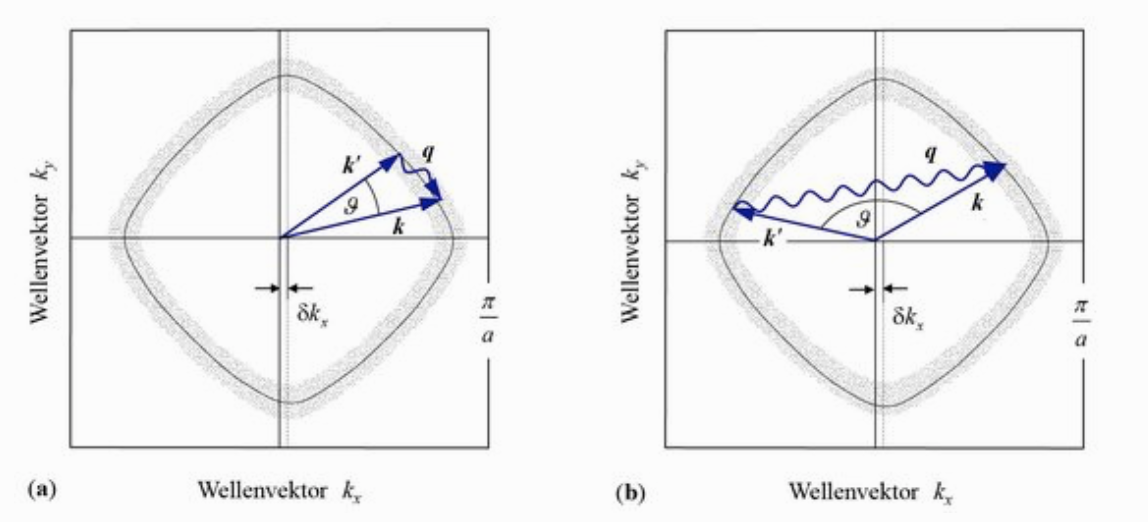
\includegraphics[width=0.6\textwidth]{streuung}
\centering
\label{fig:streuung}
\end{figure}
\subsubsection{Wärmetransport in Metallen}
Geht der Wärmetransport in erster Linie auf die Wirkung der Elektronen oder der
Phononen zurück? Bei sehr tiefen Temperaturen, liefern die Elektronen den
dominierenden Beitrag, da die spezifische Wärme der Elektronen linear mit der
Temperatur abnimmt, die des Gitter jedoch mit $T^3$ abnimmt. Wenn wir den
Beitrag der Phononen vernachlässigen, können wir für die elektronische
Wärmeleitfähigkeit $\Lambda_{el}$ wieder die Analogie zur kinetischen Gastheorie
benutzen. Da der Wärmetransport, wie der Ladungstransport nur duch angeregt
Elektronen an der Fermi-Oberfläche erfolt, können wir die spezifische Wärme und
die Fermi-Geschwindigkeit $c_V^{el}$ in $\Lambda=\frac{1}{3}Cvl$ einsetzen:
\begin{equation}
  \Lambda_{el}=\frac{1}{3}c_V^{el}vl=\frac{1}{3}\frac{\pi^2nk_B^2T}{mv_F^2}v_Fl
  =\frac{\pi^2}{3}\frac{nk_B^2\tau}{m}T
\end{equation}



\noindent \paragraph{Wiedemann-Franzsches Gesetz}
Dieses empirische Gesetz beschreibt das Verhältnis zwischen thermischer
Leitfähigkeit $\lambda$ und elektrischer Leitfähigkeit $\sigma$ als
proportiional zur Temperatur T, unabhängig von dem betrachteten Metall:
\begin{equation}
  \frac{\lambda}{\sigma}=L\cdot T
\end{equation}
Die Proportionalitätskonstante L heißt Lorenz-Zahl. Das Gesetz zeugt davon, dass
in Metallen die Ladungsträger auch Träger von Wärmeenergie sind. Es gilt für
im Vergleich zur Debye-Temperatur sehr tiefe und sehr hohe Temperaturen.
























\end{document}
